% Resultats/Distribution de sentiments


\subsection{Analyse de la Répartition des Sentiments à l'Aide de RoBERTa}
\begin{figure}[h]
    \centering
    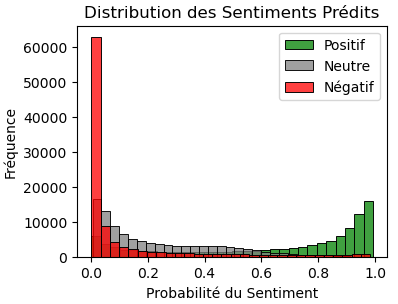
\includegraphics[scale=0.7]{assets/distributionsentimentsRoberta.PNG}
    \caption{Distribution des Sentiments Prédits}
    \label{fig:robertaSentiments}
\end{figure}
L'histogramme des probabilités de sentiments prédites révèle des tendances distinctes dans la confiance du modèle :

\begin{itemize}
    \item La catégorie 'Positif' affiche une confiance élevée, avec la majorité des probabilités concentrées dans la plage de 0.8 à 1.0.
    
    \item Pour la catégorie 'Neutre', les probabilités sont généralement plus faibles, montrant une distribution plus uniforme sur l'ensemble de la plage.
    
    \item Dans la catégorie 'Négatif', bien que des probabilités élevées soient présentes, il y a aussi une variabilité plus importante, suggérant une confiance variable dans la prédiction des sentiments négatifs.
\end{itemize}

Cette analyse détaille la diversité des confiances du modèle dans la prédiction des différents sentiments.



\subsection{Distribution des Sentiments Prédits par ROBERTA}
\begin{figure}[h]
    \centering
    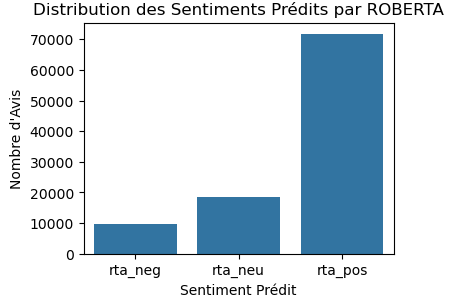
\includegraphics[scale=0.7]{assets/distributiondessentimentRoberta.PNG}
    \caption{Distribution des Sentiments Prédits}
    \label{fig:robertaSentiments}
\end{figure}

La répartition des sentiments prédits par RoBERTa sur l'ensemble de vos avis est la suivante :

\begin{itemize}
    \item \textbf{Sentiment Positif (rta\_pos)} : 71,827 occurrences
    \item \textbf{Sentiment Neutre (rta\_neu)} : 18,492 occurrences
    \item \textbf{Sentiment Négatif (rta\_neg)} : 9,607 occurrences
\end{itemize}

Cela indique que la majorité des avis ont été prédits comme ayant un sentiment positif par RoBERTa, suivi par les avis neutres, et une proportion plus faible d'avis négatifs. Cette distribution offre un aperçu de la tendance générale des sentiments dans votre ensemble de données, telle qu'interprétée par le modèle RoBERTa.


\subsection{Distribution des Sentiments ROBERTA selon les Scores}
\begin{figure}[h]
    \centering
    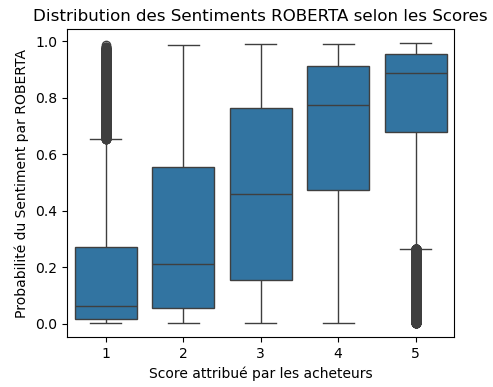
\includegraphics[scale=0.7]{assets/sentimentrobertasurscore.PNG}
    \caption{Distribution des Sentiments Prédits}
    \label{fig:robertaSentimentssurscore}
\end{figure}
On Constate que la distribution des prédictions de sentiment générées par le modèle ROBERTA, classées selon les scores attribués par les acheteurs. Les scores plus élevés tendent à avoir des prédictions de sentiment positif plus élevées, tandis que les scores plus bas montrent une variabilité plus large des prédictions. Ces informations offrent un aperçu de la corrélation entre les évaluations des acheteurs et les sentiments prédits par le modèle.



\subsection{Diagramme circulaire des proportions de sentiments}
\begin{figure}[h]
    \centering
    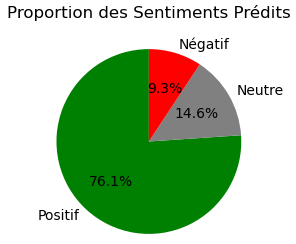
\includegraphics[scale=0.7]{assets/proportiondessentimentspredits.PNG}
    \caption{Distribution des Sentiments Prédits}
    \label{fig:proportiondessentiments}
\end{figure}

L'analyse des prédictions de sentiments révèle une tendance marquée vers des sentiments positifs, avec une majorité écrasante de 76.1\% des prédictions appartenant à cette catégorie. En revanche, les prédictions neutres sont moins fréquentes, représentant seulement 14.6\% du total. Les prédictions négatives, bien que moins prédominantes, constituent tout de même 9.3\% de l'ensemble des observations.


\subsection{Analyse des Relations entre les Probabilités Prédites et les Scores Utilisateur}

\begin{figure}[h]
    \centering
    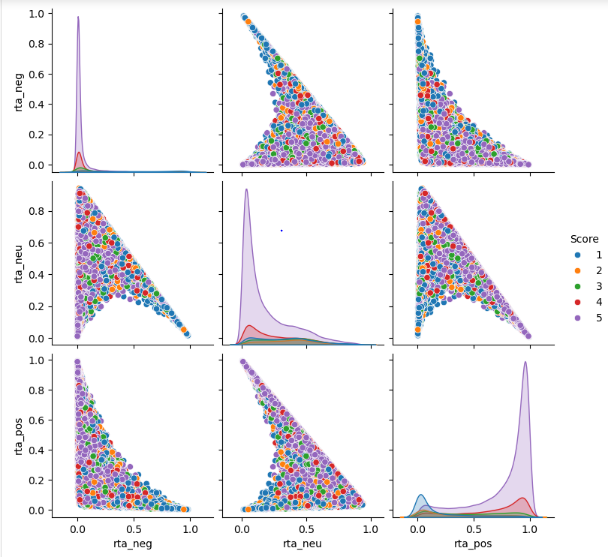
\includegraphics[scale=0.8]{assets/relation_probabilites_scores.png}
    \caption{Relation entre les Probabilités Prédites et les Scores Utilisateur}
    \label{fig:relation_probabilites_scores}
\end{figure}

L'analyse des résultats met en évidence la distribution des probabilités prédites pour chaque sentiment (négatif, neutre, positif) en fonction des scores attribués par les utilisateurs. Voici quelques observations clés :

\subsubsection{Sentiment Négatif (\texttt{rta\_neg}) :}

\begin{itemize}
    \item La probabilité moyenne de sentiment négatif augmente à mesure que le score utilisateur diminue.
    \item Les avis avec un score de 1 ont la plus grande probabilité moyenne de sentiment négatif, suivis par ceux avec un score de 2, et ainsi de suite.
    \item La dispersion des probabilités diminue à mesure que le score utilisateur augmente.
\end{itemize}

\subsubsection{Sentiment Neutre (\texttt{rta\_neu}) :}

\begin{itemize}
    \item La probabilité moyenne de sentiment neutre ne montre pas de tendance claire en fonction du score utilisateur.
    \item Les avis avec un score de 2 ont une probabilité légèrement plus élevée de sentiment neutre par rapport aux autres scores.
\end{itemize}

\subsubsection{Sentiment Positif (\texttt{rta\_pos}) :}

\begin{itemize}
    \item La probabilité moyenne de sentiment positif augmente à mesure que le score utilisateur augmente.
    \item Les avis avec un score de 5 ont la plus grande probabilité moyenne de sentiment positif.
    \item La dispersion des probabilités diminue à mesure que le score utilisateur augmente.
\end{itemize}

En résumé, le modèle RoBERTa semble bien capter la relation entre les probabilités prédites de chaque sentiment et les scores attribués par les utilisateurs. La corrélation entre la prédiction du modèle et les scores utilisateur suggère une performance raisonnable du modèle dans la classification des sentiments en fonction des avis.



\subsection{Nuage de mots des avis positifs et négatifs}


\subsubsection{Nuage de Mots pour les Avis PositifsNuage de Mots pour les Avis Positifs}
\begin{figure}[h]
    \centering
    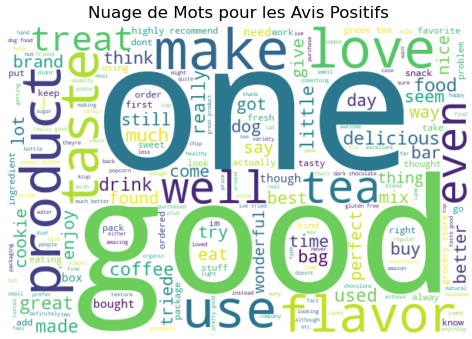
\includegraphics[scale=0.5]{assets/wordcloudpositive.PNG}
    \caption{Nuage de Mots pour les Avis Positifs}
    \label{fig:nuagepositive}
\end{figure}

Ce nuage de mots met en lumière les termes les plus fréquemment associés aux avis considérés comme positifs, tels que "good," "love," "taste," "flavor," "well," "great," et d'autres expressions positives. Ces mots reflètent les caractéristiques appréciées par les utilisateurs dans les produits alimentaires. Cette visualisation simplifiée offre un aperçu immédiat des aspects positifs saillants identifiés par le modèle dans les commentaires positifs, aidant ainsi à comprendre les tendances et les préférences des utilisateurs.


\subsubsection{Nuage de Mots pour les Avis Négatifs}

\begin{figure}[h]
    \centering
    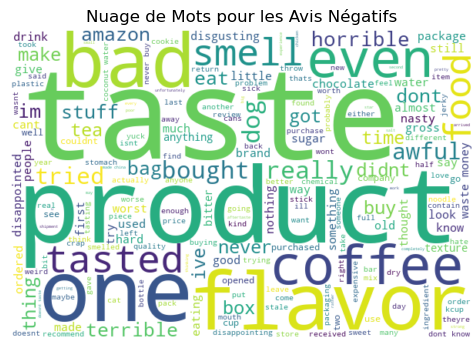
\includegraphics[scale=0.5]{assets/wordcloudnegatif.PNG}
    \caption{Nuage de Mots pour les Avis Négatifs}
    \label{fig:nuagenegatif}
\end{figure}

De manière similaire, le nuage de mots ci-dessus représente les termes les plus fréquemment associés aux avis considérés comme négatifs par le modèle RoBERTa. Certains de ces mots incluent "bad," "dont," "didnt," "horrible," "tasted," "wast money," et d'autres expressions négatives. L'analyse de ces termes permet de saisir les aspects critiques soulevés par les utilisateurs dans les avis négatifs, offrant ainsi des informations sur les points faibles perçus des produits alimentaires. Cette visualisation facilite la compréhension des motifs et des préoccupations exprimées par les utilisateurs lorsqu'ils donnent des avis négatifs.